\documentclass[11pt]{article}
\usepackage[margin=0.78in]{geometry}
\usepackage[T1]{fontenc}
\usepackage{newtxtext,newtxmath}
\usepackage{microtype}
\usepackage{xcolor}
\usepackage{graphicx}
\usepackage{float}
\usepackage{booktabs,tabularx,threeparttable}
\usepackage{fancyhdr}
\usepackage{titlesec}
\usepackage[most]{tcolorbox}
\usepackage{hyperref}
\usepackage{enumitem}
\definecolor{navy}{HTML}{17324D}
\definecolor{teal}{HTML}{167D8D}
\definecolor{coral}{HTML}{E07A5F}
\definecolor{mist}{HTML}{EFF5F7}
\definecolor{ink}{HTML}{273746}
\hypersetup{colorlinks=true,linkcolor=teal,urlcolor=teal,citecolor=teal,pdftitle={Seasonal nuisance stress evaluation for IDM-Viz}}
\graphicspath{{../../../results/phase3/seasonal_stress_reproduction_20261118_v1/analysis/}}
\pagestyle{fancy}\fancyhf{}\lhead{\small IDM-Viz | Phase 3 strengthening}\rhead{\small Seasonal stress evaluation}\cfoot{\thepage}\setlength{\headheight}{14pt}
\titleformat{\section}{\large\bfseries\color{navy}}{\thesection}{0.65em}{}[\color{teal}\titlerule]
\titleformat{\subsection}{\normalsize\bfseries\color{navy}}{\thesubsection}{0.6em}{}
\setlist{nosep,leftmargin=1.4em}
\newtcolorbox{takeaway}{colback=mist,colframe=teal,boxrule=.6pt,arc=2mm,left=2mm,right=2mm,top=1.5mm,bottom=1.5mm}
\newcommand{\StudyTag}{\textcolor{teal}{\small\bfseries POST-DEADLINE ADDITIVE STUDY \quad / \quad VERSION 1}}
\title{\vspace{-1.2em}\textcolor{navy}{Seasonal Nuisance Stress}\\[.25em]\large Paired evaluation of input alarms and frozen-model impact in IDM-Viz}
\author{IDM-Viz Phase 3 Research Implementation}
\date{18 November 2026}
\begin{document}
\maketitle\vspace{-1.2em}\begin{center}\StudyTag\end{center}
\begin{takeaway}
\textbf{Result in one sentence.} Under the configured feature-7 seasonal nuisance cycle, the input alarm rate rose sharply (paired excess about 0.74--0.77 per batch, depending on task), while the frozen classifier's paired mean accuracy change was approximately zero. This is evidence that an input alarm detects distribution movement, not evidence by itself of harmful model drift.
\end{takeaway}
\section{Why this experiment was added}
The Phase 3 configuration specified a distinct seasonal stress, but the original main runner did not permit it to execute. We repaired the runner to admit this condition only as its own stress study at the configured eight-dimensional setting. The primary eight-mechanism matrix and submitted Phase 2 methodology were not rewritten. This is a targeted implementation completion and sensitivity analysis, not a replacement of the primary matrix.

\section{Design and execution}
We used three controlled task families (linear probabilistic, nonlinear XOR, and five-region), 30 evaluation seeds per task, 96 sequential batches of 500 rows per stream, and one frozen logistic classifier per paired seed/task. The nuisance perturbation adds a sinusoid of amplitude 0.6 to feature index 7 with period 24 batches beginning at batch 1. By generator construction, this coordinate is excluded from the outcome-probability function. Each seasonal stream is paired to the stationary stream with the same task and seed, sharing the feature innovations and outcome uniforms. The analysis verified identical truth labels and checksummed all 90 seasonal cell artifacts against the run lock.

The unit of uncertainty is the seed within each task (30 paired seeds); intervals are percentile bootstrap intervals from 10,000 seed resamples. They are descriptive 95\% intervals for these generated task families. We report per-batch alarm rates averaged within a stream, then across seeds. The accuracy difference is the within-seed mean across all 96 batches for seasonal minus stationary. No threshold was tuned on this stress result.

\clearpage
\section{Results}
\begin{table}[H]
\centering\small\begin{threeparttable}
\caption{Paired seasonal-minus-stationary differences and observed alarm rates.}
\begin{tabularx}{\linewidth}{lXXX}
\toprule
Task & Accuracy difference [95\% interval] & Feature-7 alarm excess [95\% interval] & Input alarm excess [95\% interval]\\
\midrule
Linear probabilistic & $-0.00003$ [$-0.00010$, $0.00005$] & $0.791$ [$0.782$, $0.799$] & $0.744$ [$0.726$, $0.761$]\\
Nonlinear XOR & $0.00000$ [$-0.00005$, $0.00004$] & $0.791$ [$0.784$, $0.798$] & $0.768$ [$0.759$, $0.776$]\\
Five-region & $-0.00001$ [$-0.00016$, $0.00014$] & $0.795$ [$0.788$, $0.803$] & $0.764$ [$0.746$, $0.780$]\\
\bottomrule
\end{tabularx}
\begin{tablenotes}\footnotesize\item Accuracy is a fraction on a 0--1 scale. Alarm excess is the within-seed seasonal alarm rate minus the corresponding stationary rate. The seasonal feature-7 alarm rate itself was about 0.794--0.798; stationary feature-7 rates were 0.003--0.005. The overall input alarm rate was 0.803--0.811 under seasonality and 0.035--0.065 under stationarity. Intervals resample seeds within task; they do not imply generalization to arbitrary real-world seasonality.\end{tablenotes}
\end{threeparttable}
\end{table}

\begin{figure}[H]\centering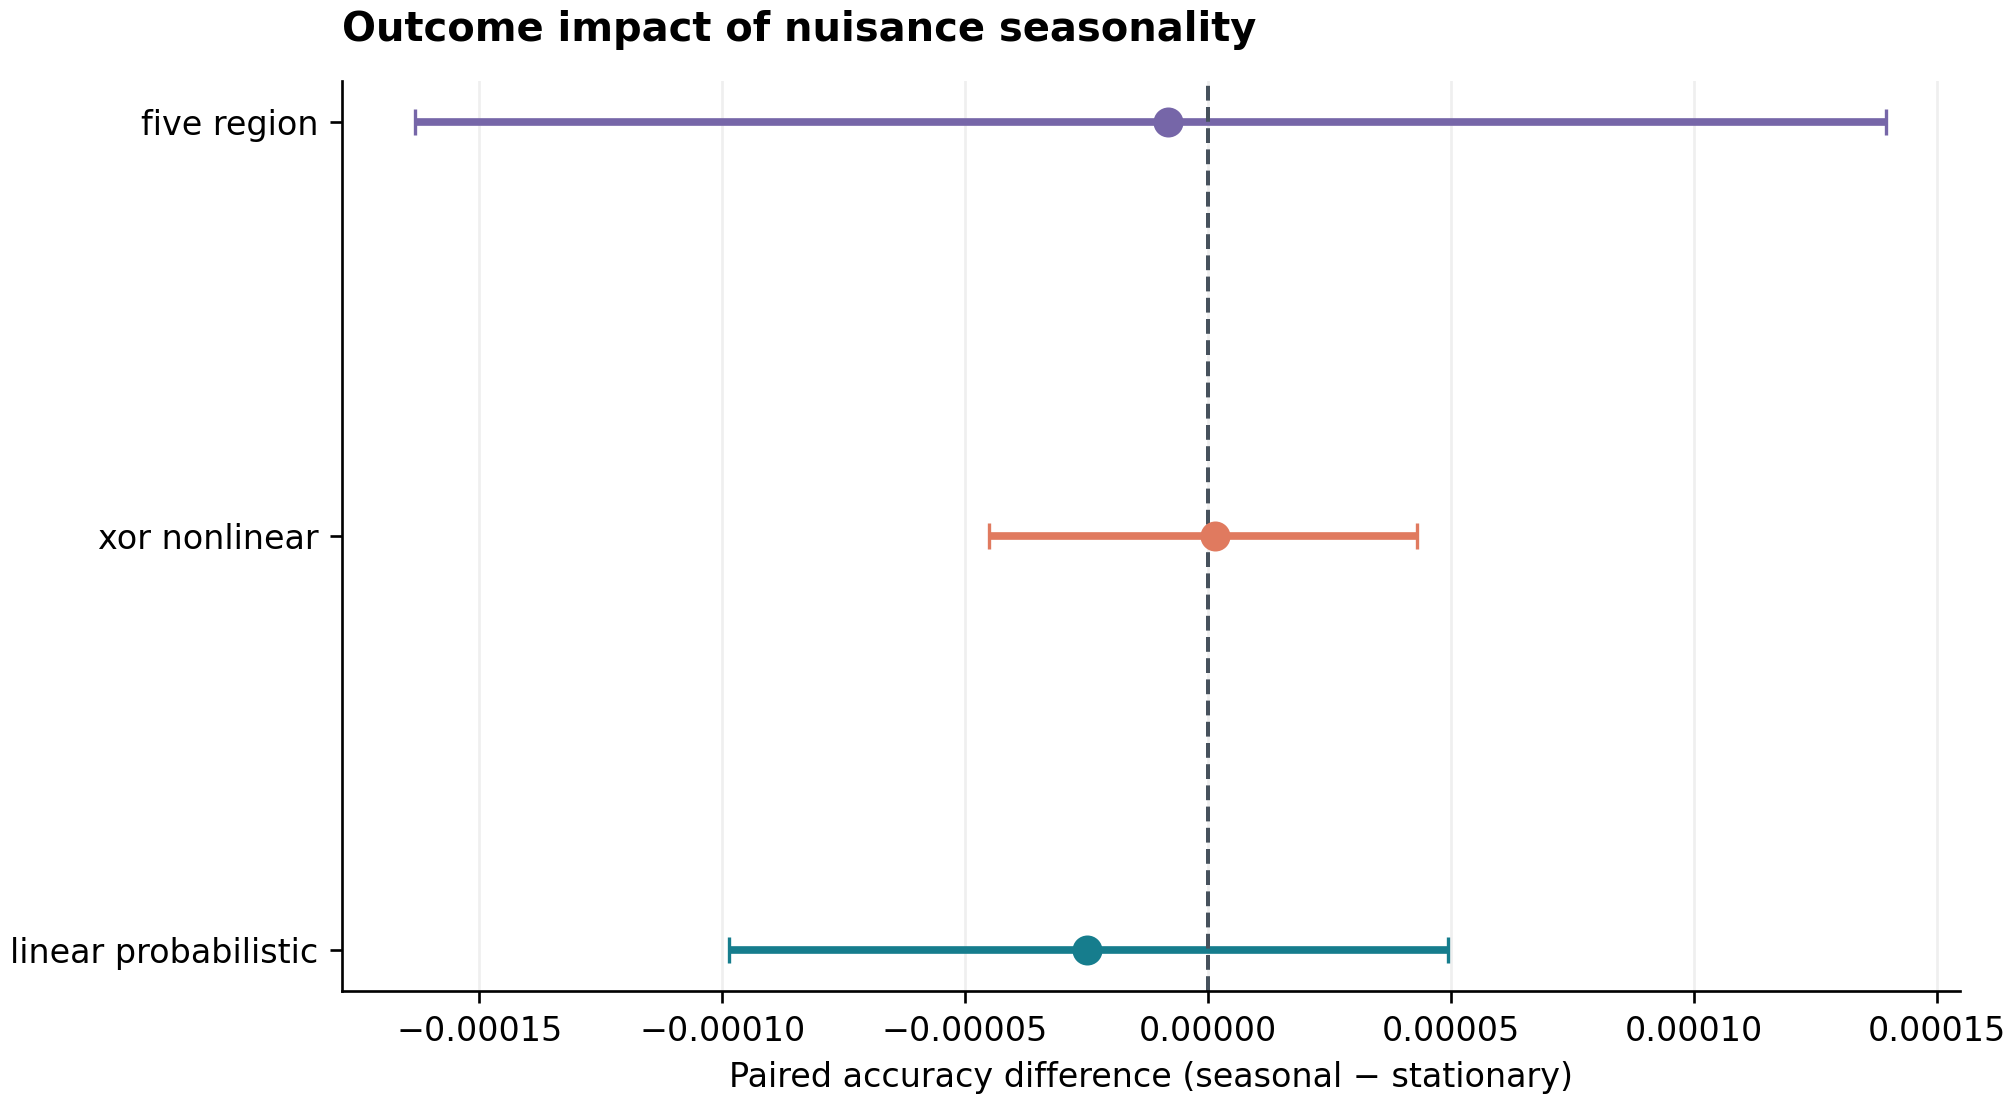
\includegraphics[width=.83\linewidth]{fig_seasonal_paired_accuracy.png}\caption{Paired seed-level accuracy change. Every task interval overlaps zero, consistent with the designed nuisance-only intervention.}\end{figure}
\begin{figure}[H]\centering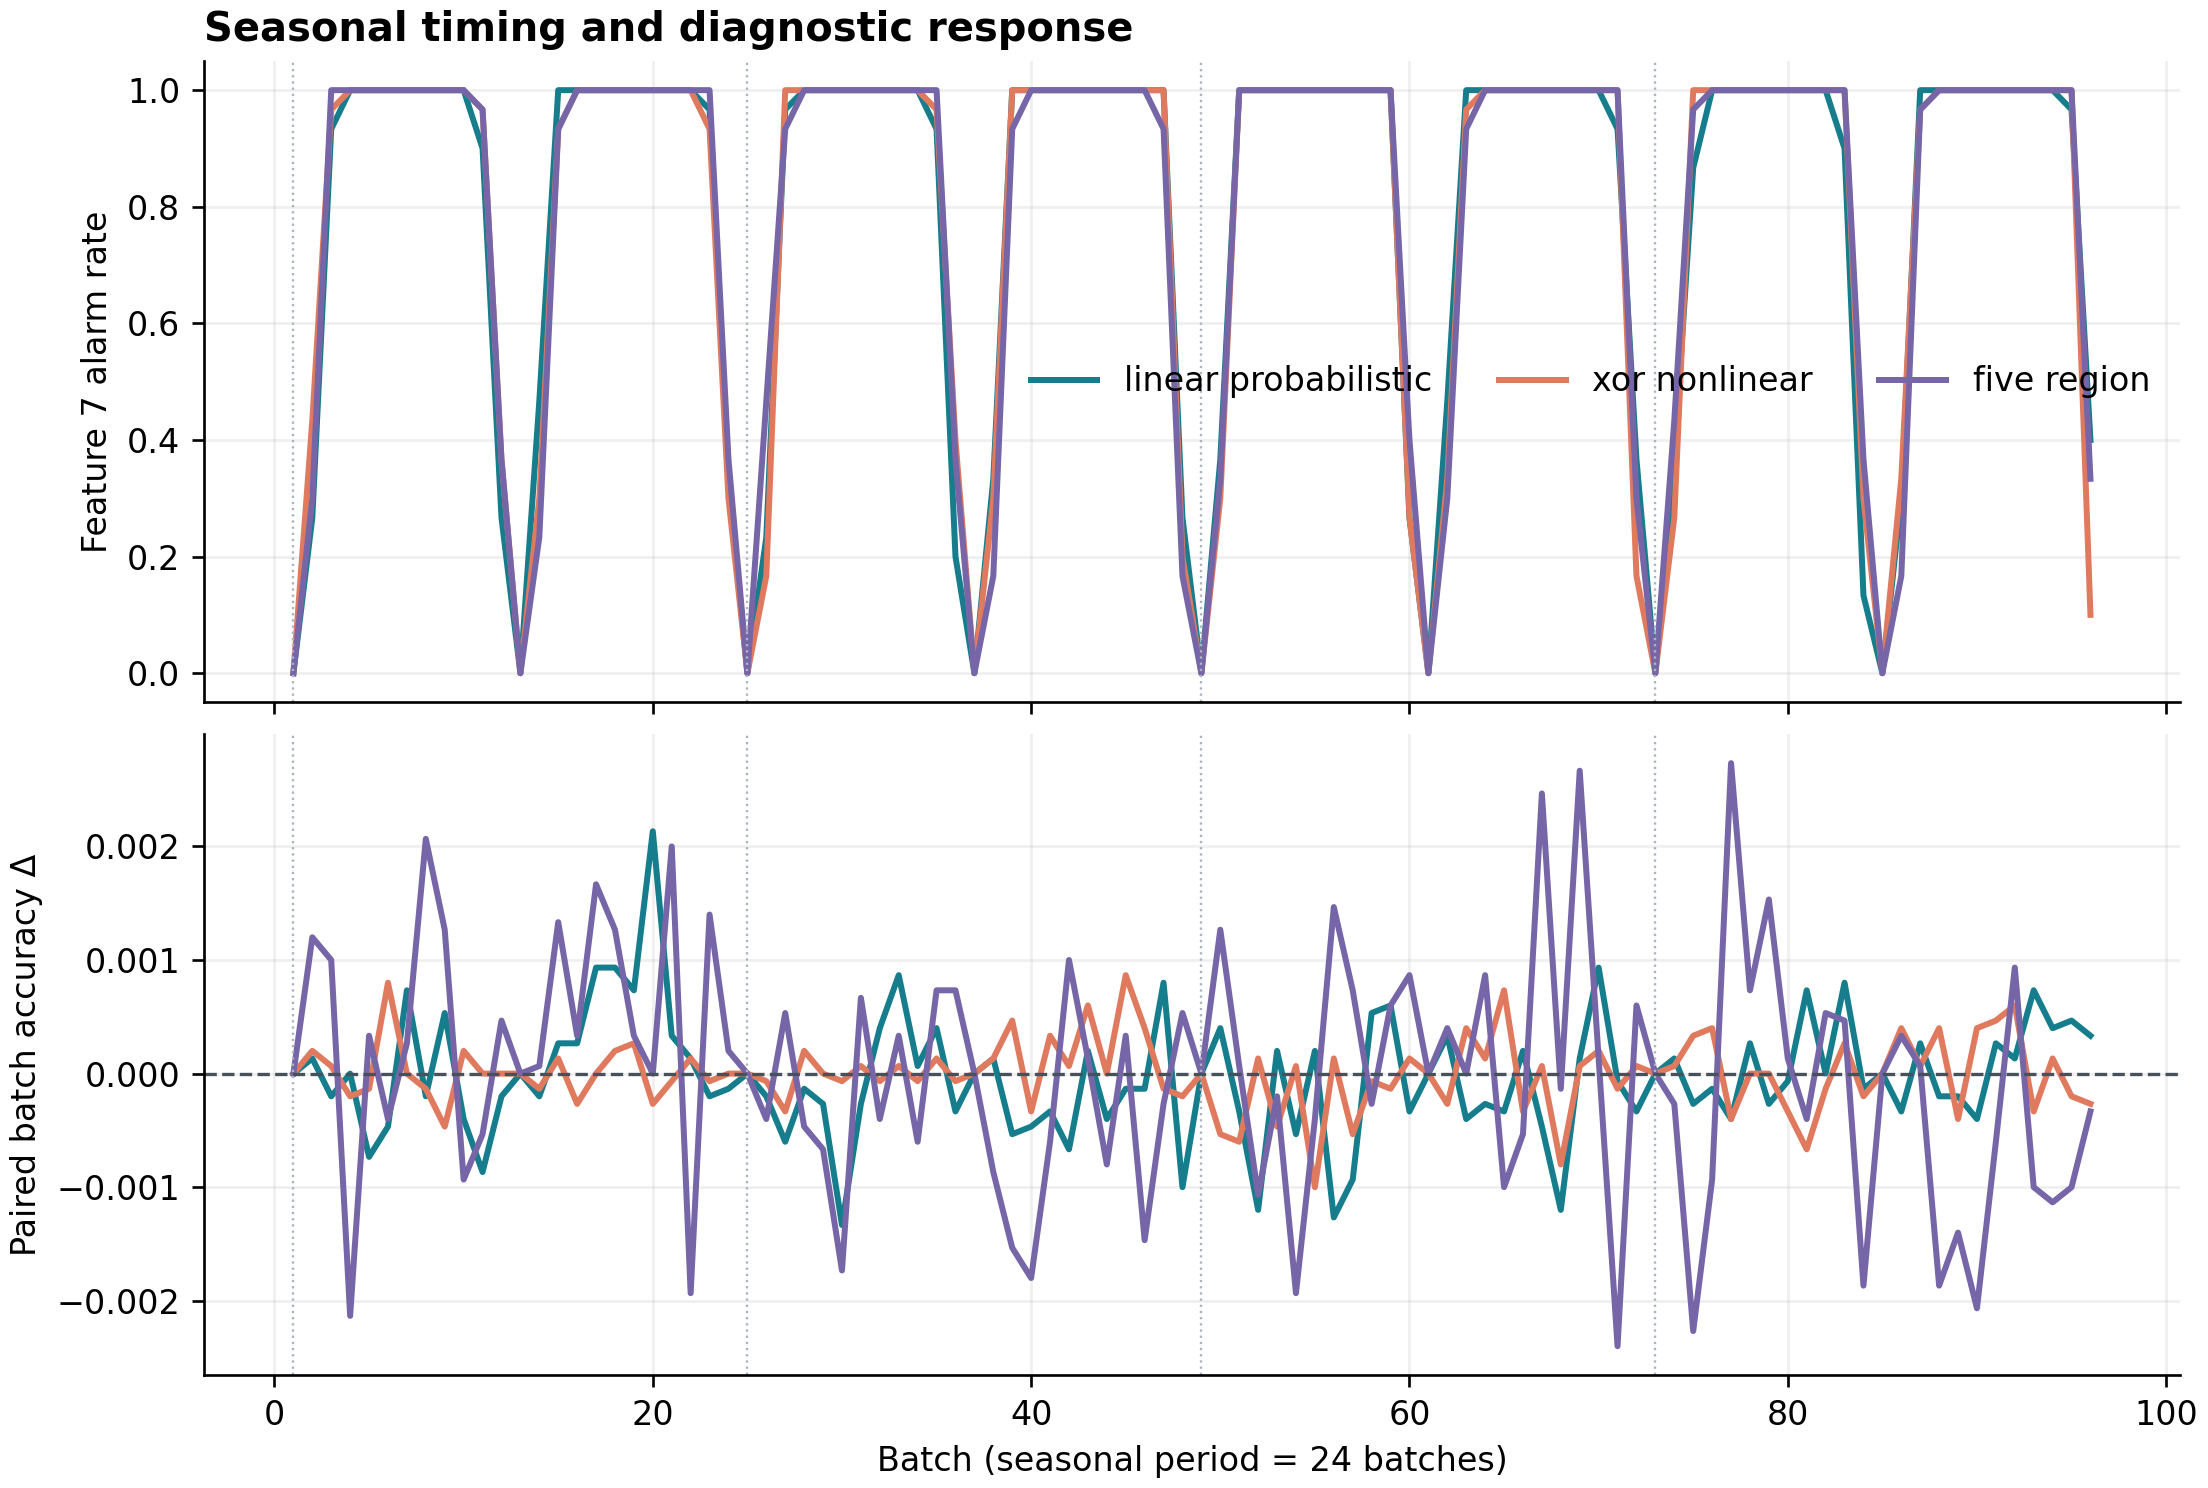
\includegraphics[width=.92\linewidth]{fig_seasonal_timeline.png}\caption{Feature-7 alarm frequency and paired batch accuracy changes over the 24-batch cycle. Feature alarms recur with the cycle while outcome impact remains centered near zero. Vertical guides mark repeated cycle boundaries.}\end{figure}

\section{Interpretation}
The detector responds strongly and cyclically to repeated input movement, but measured classifier accuracy does not meaningfully change. This is the intended negative-control behavior for separating \emph{input movement} from \emph{estimated or verified impact}. The result supports an impact-aware interpretation of alarms: users should not equate a statistically unusual feature with demonstrated model harm. At the same time, the high alarm frequency is an operational burden if the system treats every feature-distribution change as actionable.

The PCA-based alarm also fired on many batches (mean rate roughly 0.53--0.55), whereas the correlation alarm was lower (roughly 0.063--0.073). These secondary rates show that aggregation/representation changes the alarm behavior; they do not establish a universal detector ranking. Alarm rates are computed over a deliberately repeated cyclic stress and should not be compared directly to one-time abrupt-shift power without matching the event definition.

\clearpage
\section{Limitations and claims boundary}
\begin{itemize}
\item The experiment is synthetic and uses one frozen logistic model, three task families, one period and one amplitude. It does not establish robustness to real seasonal processes.
\item The assessment is paired to the stationary generator and measures detector behavior and prediction correctness; it is not a human decision-effect study, causal analysis, or proof of user benefit.
\item Evaluation seeds were already reserved for the primary protocol. The additional condition is reported as a separate, post-deadline sensitivity extension, not as an independent external replication or a silently expanded primary matrix.
\item Bootstrap intervals describe seed variation in these specified generators. They do not cover uncertainty over datasets, model classes, or seasonal mechanisms.
\item The outcome law is unchanged by design. Conclusions are therefore intentionally limited to nuisance-shift discrimination and this generator's impact response.
\end{itemize}

\section{Reproducibility}
Run from the project root with the configured Anaconda Python:
\begin{verbatim}
$py = "C:\Users\hp\anaconda3\python.exe"
& $py scripts\run_strengthening_v3.py `
  --profile evaluation `
  --task linear_probabilistic --task xor_nonlinear `
  --task five_region --mechanism S1_seasonal_nuisance `
  --dimension 8 `
  --output results\phase3\seasonal_stress_reproduction_20261118_v1
& $py scripts\analyze_seasonal_stress.py `
  --run results\phase3\seasonal_stress_reproduction_20261118_v1 `
  --primary results\phase3\strengthening_v3_evaluation_d8
& $py -m pytest -p no:cacheprovider `
  tests\phase3\test_strengthening_contracts.py `
  tests\phase3\test_strengthening_generators.py -q
& tmp\tectonic\tectonic.exe -X compile `
  reports\phase3\seasonal_stress_20261118_v1\REPORT.tex `
  --outdir reports\phase3\seasonal_stress_20261118_v1
\end{verbatim}
The independent rerun writes to a new namespace and leaves the canonical results unchanged.
The canonical run lock is recorded at:
\texttt{results/phase3/}\\
\texttt{seasonal\_stress\_evaluation\_20261118\_v1/}\\
\texttt{protocol\_lock.json}.
Canonical CSVs, plots, and hashes are in that run's \texttt{analysis/} folder. The Phase 2 DOCX remains the methodological basis and was not modified.
\end{document}

